\subsection{User Experiments}\label{subsec:userexp}

The entire system have been tested through an end user experiment involving a subset of the users. The experiment includes 10 drivers, who have been instructed to use the system for all their vehicular trips. To get started, all users received a two-page guide for setting up Drive-LaB on their smartphone. This guide can be seen in Section \ref{appendix:drivelab_guide} in Appendices. The experiment ran from the 1st of May till the 3rd of June. As a motivator for using the system thoroughly, a competition was hosted, offering a prize for the user with the lowest average score percentage. The competition could be followed live through the application, allowing the drivers to monitor current results and compare them with other participants. At the end of the competition the 10 users completed 345 trips spanning 8.191 kilometers.

\begin{figure*}[tb]
\centering
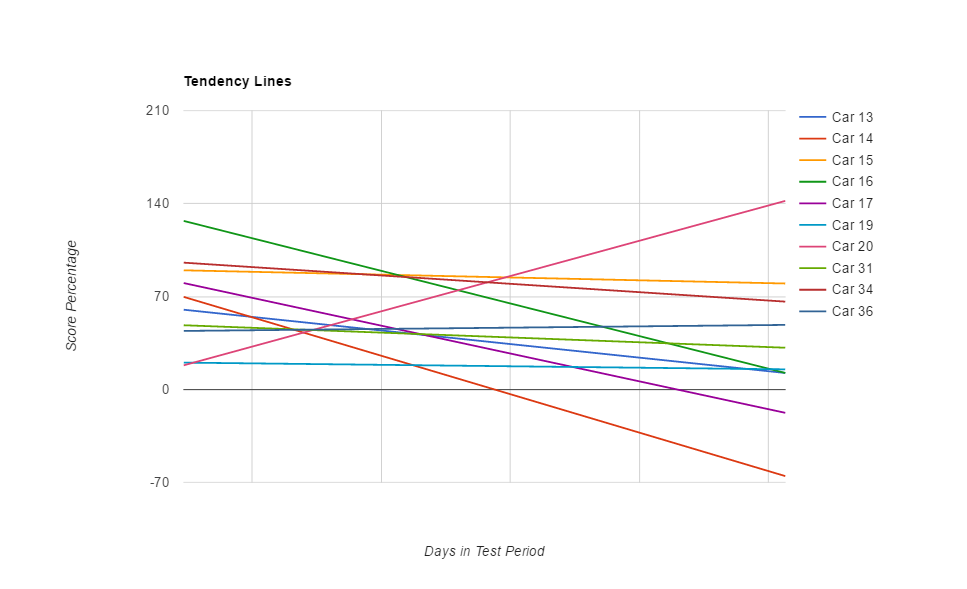
\includegraphics[width=0.95\textwidth]{Pictures/tendenslinjer}
\caption{A line chart showing the tendency lines for each individual driver}
\label{fig:tendencylines}
\end{figure*}

There are several points to asses in this experiment, and one of them is to test the system in its entirety, in a setting true to the environment where the system is eventually going to be release in. This test setup is as true to the real setting as possible. The frontend application was deployed on Google Play, where the test subjects downloaded and started to use the product. Throughout the experiments, they were presented with a leaderboard with average scores for each of all the drivers. 
It would be desirable to receive user inputs on the system, whether it is easy to use or there are some obvious improvements to make. However, the user feedback is still on its way.

One of the more interesting things to investigate through this experiment, is whether or not there is any improvement in score percentages for each driver. Figure \ref{fig:tendencylines} shows the tendency lines for each of the driver throughout the test period. It is important to notice this is merely tendency lines and not projection lines. Figure \ref{fig:tendencylines} shows a downward trend with 8 of the 10 drivers, with slope ratios between -0,284 and 3,273. It shows an upward trend with the last 2 driver, with slope ratios at 0,13 and 3,54. The highest numerical slope ratios are representing the drivers with the fewest amount of trips, and drivers with 0 trips later in the test period. What these results reveal, is that users of the system scores slightly better when having used the system for a period of time. This could mean that users of the system drives better and better dependent on the system indicating when they are actually a good driver.

%\begin{figure*}[tb]
%\centering
%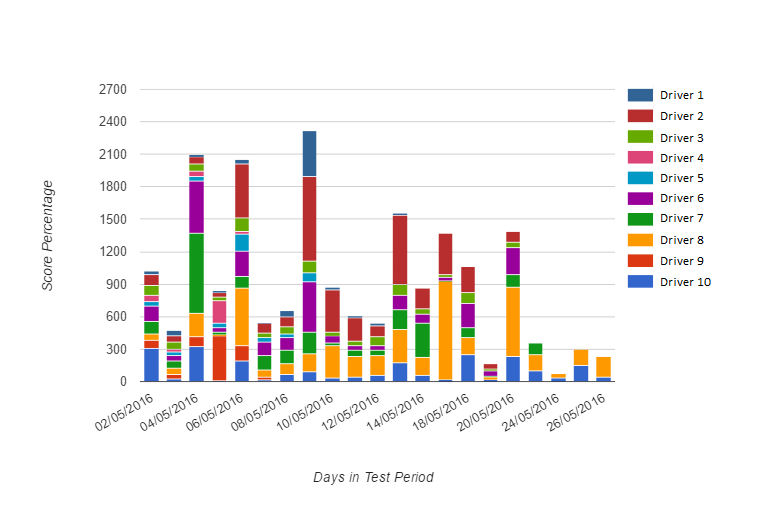
\includegraphics[width=0.95\textwidth]{Pictures/summationoftripscore}
%\caption{A summation of scores based on days}
%\label{fig:summationoftripscore}
%\end{figure*}

Lastly, there is an interesting point to whether or not there is an incentive to keep using the system. As mentioned, the winner of the experiment were to receive a prize at the end. As shown in Figure \ref{fig:summationoftripscore} there is a slight negative tendency in score summation, but it roughly correlates with the negative slope ratios of the tendencies in trip percentages. This means there was incentive enough to keep using the system, with the given prize. In a future insurance environment the incentive would be a cheaper insurance for the end user -therefore given the monetary value roughly equals the prize of the experiment, that should be plentiful incentive.
 